\documentclass[journal]{IEEEtran}

\usepackage{amsmath,amssymb,amsfonts}
\usepackage{booktabs}
\usepackage{tabularx}
\usepackage{graphicx}
\usepackage{cite}
\usepackage{url}
\usepackage{microtype}
\usepackage{seqsplit}

\begin{document}

\title{WHOT-ML: A Configurable Partially Observable Multi-Agent Environment for Machine Learning Research}

\author{Brayan~Osinaka%
\thanks{Manuscript received November 3, 2026; revised November 13, 2026. Brayan Osinaka is an independent researcher based in Benin City, Edo State, Nigeria (e-mail: brayanjunior101@gmail.com). Source code and trajectory datasets are archived under DOI: 10.5281/zenodo.23918026.}}

\markboth{IEEE Transactions on Games,~Vol.~X, No.~X,~November~2026}%
{Osinaka: WHOT-ML: A Configurable Partially Observable Multi-Agent Environment}

\maketitle

\begin{abstract}
Multi-agent reinforcement learning (MARL) in imperfect-information games often exhibits pathological equilibrium behaviors, including defensive retaliation loops, coordination collapses, and ungrounded belief dynamics. While benchmarks such as Poker and Hanabi have advanced imperfect-information reasoning, they focus predominantly on two-player zero-sum betting or cooperative communication with inverted visibility. We introduce WHOT-ML, an open-source, deterministic benchmark formalizing the Nigerian card game WHOT as a Partially Observable Stochastic Game (POSG) featuring non-uniform deck topologies, multi-card penalty stacking, dynamic action masking, and concealed draw decks. Through an extensive empirical campaign spanning 16,850 games executed in containerized cloud infrastructure, we uncover two foundational phenomena. First, symmetric heuristic self-play induces an emergent defensive stall (43.6\% truncation rate) driven by retaliatory penalty looping and market recycling. Second, a Masked Proximal Policy Optimization (PPO) baseline completely resolves this coordination failure, collapsing truncations to 0.5\% and shortening game duration from 506.4 to 141.1 turns. Furthermore, diagnostic linear probing of the frozen policy trunk reveals that feedforward representations implicitly construct probabilistic belief states over unobserved opponent hands (mean AUROC 0.597, conditional AUROC 0.532 on unseen cards) without explicit recurrent memory. WHOT-ML provides a mathematically rigorous, bitwise-reproducible laboratory for studying strategic coordination, defensive stalls, and belief-state inference in multi-agent systems.
\end{abstract}

\begin{IEEEkeywords}
Multi-agent reinforcement learning, partially observable stochastic games, imperfect-information games, benchmark environments, emergent defensive stalls, latent belief probing.
\end{IEEEkeywords}

\section{Introduction}
\IEEEPARstart{A}{utonomous} decision-making in multi-agent domains frequently requires agents to act under severe information asymmetry, hidden state transitions, and competitive friction. In real-world environments—such as financial auctions, autonomous transport coordination, cyber-physical defense, and strategic negotiation—agents rarely observe the ground-truth state of their environment. Instead, they must filter public event histories into private belief representations, anticipate the hidden intentions of competitors, and select actions under combinatorial uncertainty \cite{kaelbling1998planning,hansen2004dynamic}.

Games have long provided foundational proving grounds for artificial intelligence, driving breakthrough advances from perfect-information board games such as Chess and Go \cite{silver2018general} to imperfect-information card games such as Poker \cite{bowling2015heads,moravcik2017deepstack,brown2018superhuman,brown2019superhuman} and Hanabi \cite{bard2020hanabi}. However, existing imperfect-information benchmarks concentrate on specialized game structures. Poker centers primarily on two-player, zero-sum betting with static deals, lacking spatial matching mechanics or dynamic turn modifications. Hanabi emphasizes purely cooperative communication under inverted visibility, where agents view only teammate hands. Meanwhile, popular shedding games such as Uno, Crazy Eights, and Dou Dizhu \cite{zha2020rlcard,zha2021douzero} feature simplified matching rules or asymmetric bidding roles that omit the complex multi-card penalty stacking chains, compulsory declaration penalties, and cyclical deck recycling common to indigenous shedding traditions.

To bridge this methodological gap, we introduce \textbf{WHOT-ML}, a computational research environment based on the national card game of Nigeria, WHOT. Played with a specialized 54-card deck comprising five non-uniform geometric suits (Circle, Triangle, Cross, Square, Star) and five wild WHOT cards, the game combines shape and number matching with powerful action cards that repeat turns (Hold On), skip opponents (Suspension), compel adversaries to draw penalty cards (Pick Two, Pick Three), demand table-wide card draws (General Market), or declare new active suits (WHOT). Crucially, players hold private hands, draw from a hidden market deck, and face strict penalty enforcement if they fail to announce their penultimate card before victory (Last Card). 

In multi-agent environments with defensive mechanics, greedy heuristic policies often produce severe coordination failures. When players counter attacks with retaliatory defenses, accumulated card penalties can overwhelm draw decks, forcing continuous discard pile recycling that traps agents in endless defensive loops. Understanding whether learned policies can discover cooperative pressure, sacrifice plays, or offensive tempo to escape such defensive stalls is a core open question in multi-agent reinforcement learning (MARL). Simultaneously, identifying whether feedforward deep policies can implicitly maintain probabilistic representations of hidden state without recurrent memory structures provides critical insights into representation learning under partial observability.

This work makes four principal contributions. First, we mathematically formalize WHOT as a finite-horizon, turn-based Partially Observable Stochastic Game (POSG) with perfect recall and dynamic action masking, implemented in an open-source, bitwise-deterministic reference simulator (\texttt{WHOT-NG-v1.0.1}) that achieves a certified 100.0\% Reproduction Success Rate. Second, we empirically prove that partial observability is operationally consequential: evaluating 449 observationally equivalent state pairs reveals an 84.63\% trajectory divergence rate under deterministic rollouts ($p < 10^{-15}$). Third, across an empirical campaign of 16,850 cloud-executed production runs, we discover an emergent defensive stall in symmetric heuristic self-play (43.6\% truncation rate) and uncover a structural scaling regime shift governed by the card depletion ratio $\rho_0 > 1.0$. Fourth, we implement and train a Masked Proximal Policy Optimization (PPO) baseline for 10M environment timesteps, demonstrating that learned self-play decisively overcomes the defensive stall (reducing truncations to 0.5\% and shortening game duration by 72.1\%), while diagnostic linear probing confirms that feedforward policy trunks implicitly infer unobserved opponent card distributions (mean AUROC 0.597, conditional AUROC 0.532 on unseen cards) purely from public action histories.

\section{Related Work}
Extensive-form games with imperfect information are formalized theoretically as Partially Observable Stochastic Games (POSGs) \cite{hansen2004dynamic} or Markov games \cite{littman1994markov}. While standard single-agent POMDPs require maintaining a belief state over world configurations \cite{kaelbling1998planning}, multi-agent POSGs require reasoning over opponent information sets $\mathcal{I}_i$, private strategies, and non-stationary environment transitions. In WHOT-ML, the number of distinct partitions of 47 unobserved cards across three opponent hands of 6 cards and a 29-card draw market equals $\frac{47!}{(6!)^3 \cdot 29!} \approx 7.8 \times 10^{13}$. This generates a combinatorial hidden belief space exceeding $10^{13}$ states consistent with a single opening observation.

Imperfect-information game benchmarks have historically catalyzed algorithmic breakthroughs. Heads-up and multiplayer No-Limit Texas Hold'em enabled superhuman achievements through Counterfactual Regret Minimization (CFR) and recursive depth-limited solving \cite{bowling2015heads,moravcik2017deepstack,brown2018superhuman,brown2019superhuman}. Hanabi established a premier cooperative benchmark for theory of mind and communicative convention emergence \cite{bard2020hanabi}. In card shedding, DouZero demonstrated that deep reinforcement learning can master complex combinations in Dou Dizhu \cite{zha2021douzero}. Standardized simulation suites such as OpenAI Gym \cite{brockman2016openai}, PettingZoo \cite{terry2021pettingzoo}, OpenSpiel \cite{lanctot2019openspiel}, and RLCard \cite{zha2020rlcard} provide multi-agent environments, but focus predominantly on standard Anglo-American decks or fixed rule configurations. WHOT-ML complements these testbeds by introducing non-uniform suit distributions, cumulative penalty stacking chains, compulsory declaration penalties, and a modular rules engine supporting programmatic ablations.

\section{WHOT-ML Environment}
The game of WHOT is played with a canonical 54-card deck comprising five geometric suits and wild cards: $\mathcal{C}_{54} = \mathcal{C}_{\text{Circle}} \cup \mathcal{C}_{\text{Triangle}} \cup \mathcal{C}_{\text{Cross}} \cup \mathcal{C}_{\text{Square}} \cup \mathcal{C}_{\text{Star}} \cup \mathcal{C}_{\text{WHOT}}$. The deck features a distinct non-uniform distribution across suits: Circle and Triangle contain 12 cards each ($\{1, 2, 3, 4, 5, 7, 8, 10, 11, 12, 13, 14\}$); Cross and Square contain 9 cards each ($\{1, 2, 3, 5, 7, 10, 11, 13, 14\}$); Star contains 7 cards ($\{1, 2, 3, 4, 5, 7, 8\}$); and WHOT contains 5 wild cards of face value 20. In the reference configuration, each player is dealt $H_0 = 6$ private cards. One card is dealt face-up to establish the discard play pile, while the remaining 29 cards form the face-down draw market.

We formalize WHOT-ML as a turn-based Partially Observable Stochastic Game with finite horizon $T_{\max}=1{,}000$ and perfect recall, defined by the tuple $\mathcal{G} = \langle \mathcal{N}, \mathcal{S}, \mathcal{A}, \mathcal{O}, \mathcal{T}, \Omega, \mathcal{R}, \gamma \rangle$, where $\mathcal{N} = \{0, 1, \dots, N-1\}$ is the player set ($N \in \{2..6\}$); $\mathcal{S}$ is the complete world state space; $\mathcal{A}$ is the joint action space; $\mathcal{O}$ is the observation space; $\mathcal{T}: \mathcal{S} \times \mathcal{A} \to \Delta(\mathcal{S})$ is the transition probability function; $\Omega_i: \mathcal{S} \to \mathcal{O}_i$ is the private observation function for player $i$; $\mathcal{R}_i: \mathcal{S} \times \mathcal{A} \to \mathbb{R}$ is the reward function; and $\gamma \in (0, 1]$ is the discount factor.

The complete state $S_t \in \mathcal{S}$ is fully specified by $S_t = \langle \mathbf{H}_t, M_t, D_t, c_t, p_t, \pi_t, \delta_t, \mathbf{L}_t, t, \mathcal{C}_{\text{config}} \rangle$, where $\mathbf{H}_t = (H_t^0, \dots, H_t^{N-1})$ denotes the private hand multisets; $M_t = [m_1, \dots, m_k]$ is the ordered market deck; $D_t = [d_1, \dots, d_m]$ is the discard pile with active top card $d_m$; $c_t \in \{\text{Circle}, \text{Triangle}, \text{Cross}, \text{Square}, \text{Star}\} \cup \{\emptyset\}$ is the active nominated suit; $p_t \in \mathcal{N}$ is the active turn player; $\pi_t \in \mathbb{N}_{\ge 0}$ is the accumulated penalty counter; $\delta_t \in \{+1, -1\}$ is the play direction; $\mathbf{L}_t \in \{0, 1\}^N$ is the vector of last-card declaration flags; $t \in \mathbb{N}$ is the turn counter; and $\mathcal{C}_{\text{config}}$ is the immutable configuration parameter set.

The discrete action space $\mathcal{A}$ contains 76 discrete slots: Indices 0--48 map to normal physical card plays in canonical deck order; Indices 49--73 map to WHOT wild card plays paired with one of five ordinary shape nominations ($5 \text{ WHOT cards} \times 5 \text{ shapes} = 25$ actions); Index 74 represents the market draw action (\texttt{DRAW}); and Index 75 represents the last-card declaration action (\texttt{DECLARE\_LAST}). To ensure valid transitions, the environment emits a dynamic boolean action mask $\mathbf{m}_t \in \{0, 1\}^{76}$. A normal card play is legal if its suit or face value matches the active discard $d_m$, or matches the active nominated shape $c_t$ when a WHOT card is active. Wild WHOT cards (value 20) are legal on any normal card and require declaring a follow-up suit. If an active penalty exists ($\pi_t > 0$), the acting player may only play a matching defense card to stack the penalty or execute \texttt{DRAW} to absorb the accumulated cards. Drawing is unconditionally legal on any turn, even if playable cards are held.

The \texttt{DECLARE\_LAST} action formalizes the cultural ``Last Card'' rule, becoming legally available when a player holds exactly two cards prior to play (or one card upon completion) and has not yet declared. In the default configuration, executing \texttt{DECLARE\_LAST} does not consume the player's turn; the player sets their declaration flag and retains priority to shed their card. Conversely, shedding the final card without prior declaration triggers an undeclared victory violation: shedding victory is denied, the violator draws penalty cards (1 card in baseline, 2 under \texttt{VAR-PENALTY-2}), and play advances.

The observation function $O_t^i = \Omega_i(S_t)$ enforces strict information boundaries: $O_t^i = \langle H_t^i, d_m, c_t, p_t, \pi_t, \mathbf{h}_t, |M_t|, \mathbf{L}_t, \mathcal{H}_t^{\text{public}}, \mathbf{m}_t^i \rangle$, where $H_t^i$ is player $i$'s private hand, $\mathbf{h}_t = (|H_t^0|, \dots, |H_t^{N-1}|)$ is the public hand size vector, $|M_t|$ is the scalar market card count, and $\mathcal{H}_t^{\text{public}}$ is the sequence of public discards, calls, and draw events. The observation exposes strictly zero information regarding opponent card identities or market sequence.

Six special card values govern environment dynamics: Hold On (Card 1) grants an immediate repeat turn; Pick Two (Card 2) compels the next player to draw 2 cards, which may be countered with another Pick Two under penalty stacking to accumulate $\pi \leftarrow \pi + 2$; General Market (Card 14) forces all opponents to draw 1 card; Suspension (Card 8) skips the next player; Pick Three (Card 5) compels the next player to draw 3 cards; and WHOT (Card 20) serves as a wild card declaring the active suit. When the draw market is depleted ($|M_t| = 0$), the discard pile is preserved at top card $d_m$, while cards $[d_1, \dots, d_{m-1}]$ are collected, deterministically reshuffled, and reconstituted as the new market $M_{t+1}$. A game terminates when a player sheds their final card ($|H^i|=0$), awarding $+1.0$ to the winner and $-1.0$ to losing players, or truncates upon reaching $T_{\max} = 1{,}000$ turns without a victor.

\section{Experimental Methodology}
The reference simulator \texttt{WHOT-NG-v1.0.1} is verified against a 114-test regression suite ensuring card conservation invariants and strict observation isolation. Across 200 independent trials (100 full-game replays and 100 mid-game JSON checkpoint restorations), the simulator achieves a 100.0\% Reproduction Success Rate, generating bitwise identical SHA-256 state digests that certify zero-drift determinism for reinforcement learning rollouts.

Two non-learning reference policies establish foundational benchmarks. \texttt{RandomLegalAgent} samples uniformly from the active action mask $\mathbf{m}_t(S_t)$, defining the stochastic performance floor. \texttt{RuleBasedAgent} implements an aggressive domain heuristic: it declares last-card immediately when eligible; prioritizes counter-defense over drawing when facing active penalties; greedily fires high-impact special attack cards in strict priority order (Hold On, General Market, Suspension, Pick Two/Three, and ordinary matching cards) rather than conserving them; nominates the most frequent suit in hand when playing WHOT cards; and resolves candidate action ties deterministically by canonical hand order.

To ensure computational independence from local development machines, the production workload of 16,850 games (14,850 baseline games, 2,000 PPO evaluation games, and 10,000 latent probes) was packaged, dispatched via API, and executed on containerized Kaggle Cloud Linux instances (kernel 6.6.137+, Python 3.13.15, NVIDIA T4/P100 GPUs, total compute time 6.87 GPU hours). All raw trajectory artifacts were archived with cryptographic SHA-256 hashing.

Statistical inference relies on unpooled, game-level Wilson score 95\% confidence intervals \cite{wilson1927probable} for binomial proportions (win rates, truncation frequencies, divergence rates). Continuous metric distributions are reported via means, standard deviations, medians, and interquartile ranges [IQR]. Distributional shifts across rule ablations are quantified via Cliff's delta effect size ($\delta \in [-1, +1]$) \cite{cliff1993dominance}, and seating balance is verified via Pearson's chi-square test ($\chi^2$).

\begin{table}[t]
\centering
\caption{WHOT-NG-v1 Baseline Characterization (EXP-01, $N = 2{,}000$ Episodes)}
\label{tab:exp01_characterization}
\small
\resizebox{\columnwidth}{!}{%
\begin{tabular}{lccc}
\toprule
\textbf{Metric} & \textbf{RandomLegal} & \textbf{RuleBased} & \textbf{Space / Bound} \\
\midrule
Physical Cards ($N_{\text{deck}}$) & 54 & 54 & 54 Cards \\
Action Space ($|\mathcal{A}|$) & 76 & 76 & 76 Slots \\
Legal Actions (Mean $\pm$ SD) & 2.42 $\pm$ 2.40 & 7.63 $\pm$ 7.11 & Masked \\
Legal Actions (Median [IQR]) & 1.0 [1.0, 3.0] & 5.0 [2.0, 11.0] & Masked \\
Game Duration (Mean Turns) & 368.3 & 506.4 & Max 1,000 \\
Game Duration (Median [IQR]) & 270.5 [125.8, 546.2] & 248.0 [75.8, 1000.0] & Max 1,000 \\
Mean Draws per Game & 245.3 & 457.7 & Open Market \\
Market Reshuffles per Game & 8.19 & 270.36 & Recycled \\
Declaration Violations & 1,079 & 0 & Heuristic Inv. \\
Truncation Rate [95\% CI] & 7.6\% [6.1\%, 9.4\%] & 43.6\% [40.6\%, 46.7\%] & 1,000 Turns \\
\bottomrule
\end{tabular}%
}
\end{table}

\begin{figure}[t]
\centering
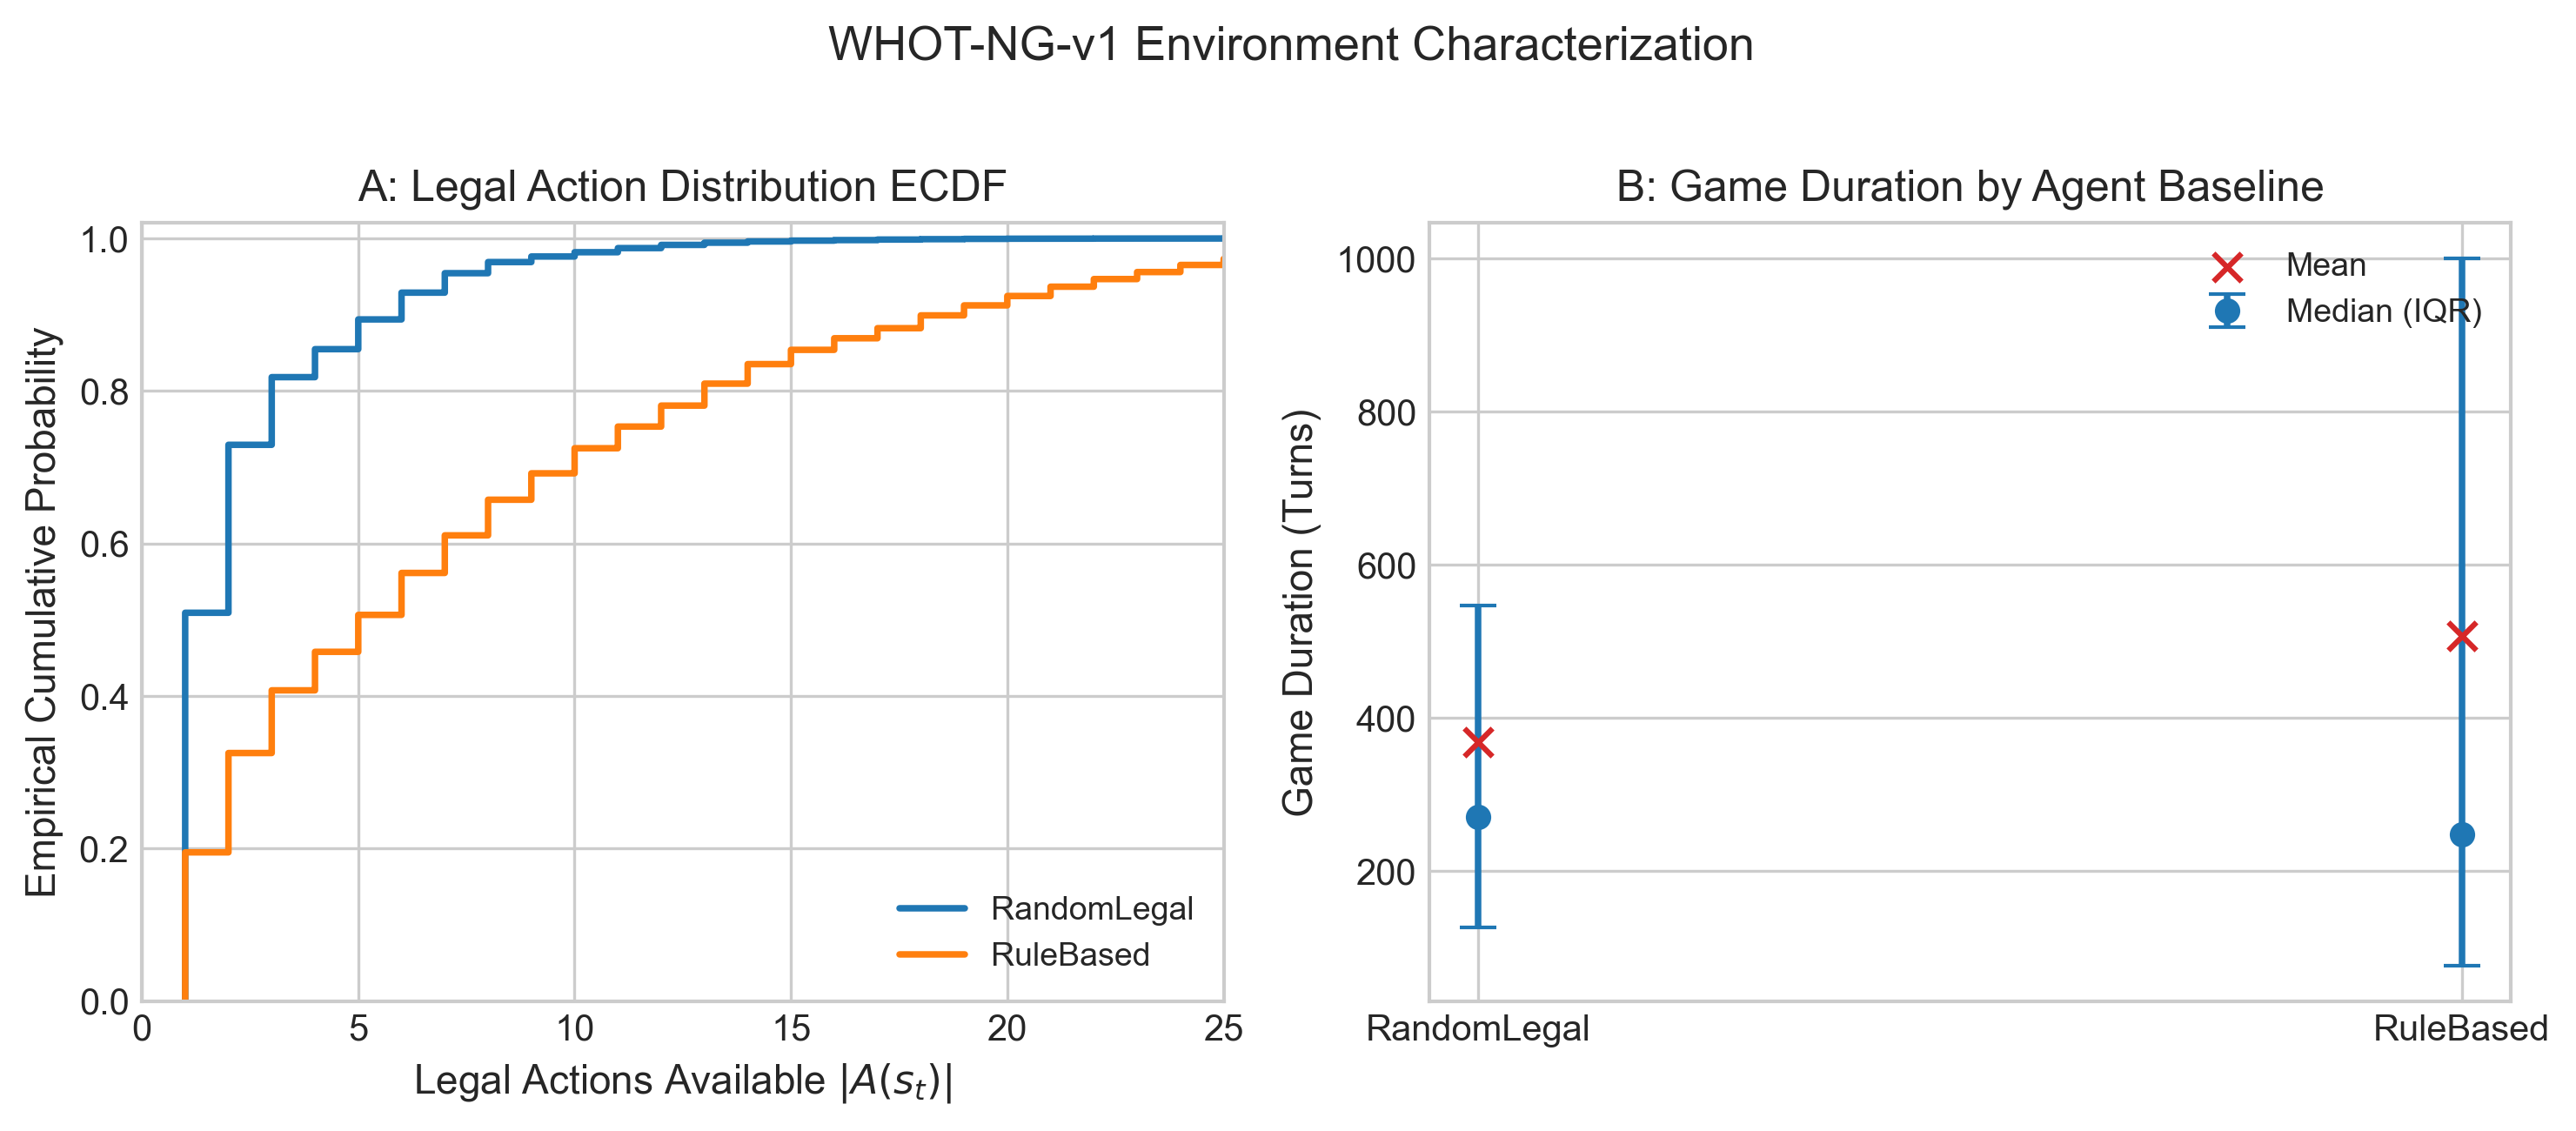
\includegraphics[width=\columnwidth]{figures/fig1_characterization_full.png}
\caption{Environment Characterization under Baseline Agents (EXP-01). (a) Empirical Cumulative Distribution Function of legal actions $|\mathcal{A}(S_t)|$. (b) Game duration distributions across 1,000 games per cohort.}
\label{fig:fig1_characterization}
\end{figure}

\section{Baseline Characterization and Partial Observability}
We characterize the environment baseline across 2,000 4-player games ($H_0 = 6$) divided into two cohorts of 1,000 games each: Cohort 1 evaluated four \texttt{RandomLegalAgent} players (seeds 10000--10999), while Cohort 2 evaluated four \texttt{RuleBasedAgent} players (seeds 11000--11999), encompassing 874,732 logged decision steps (Table~\ref{tab:exp01_characterization} and Figure~\ref{fig:fig1_characterization}).

A critical phenomenon emerges in Cohort 2: while random games truncate at a modest 7.6\% rate with an average of 8.19 market reshuffles, symmetric heuristic self-play (\texttt{BBBB}) triggers a massive \textbf{43.6\% truncation rate} [40.6\%, 46.7\%] with an average of \textbf{270.36 market reshuffles} and 457.7 card draws per game. Event log auditing reveals that this emergent defensive stall is driven by defensive symmetry: when Player A attacks with a Pick Two, Player B counters with another Pick Two, transferring a 4-card penalty to Player C. When an attacked player cannot counter, they absorb massive card draws, rapidly depleting the market. Discard recycling subsequently returns these special cards into the draw deck. Because greedy agents aggressively fire special attacks and immediately play matching counter-defenses, the game becomes trapped in an oscillatory loop where penalty cards repeatedly exhaust and recycle the market deck between hands and draw market without reaching completion. Escaping this coordination stall requires strategic sacrifices and card-dumping sequences that greedy heuristics cannot discover.

\begin{table}[t]
\centering
\caption{Partial Observability Trajectory Divergence (EXP-02, $N = 449$ State Pairs)}
\label{tab:exp02_partial_observability}
\small
\resizebox{\columnwidth}{!}{%
\begin{tabular}{lcc}
\toprule
\textbf{Metric} & \textbf{Empirical Value} & \textbf{Formal Bound} \\
\midrule
Observation Equivalence Rate & 100.0\% & 100.0\% ($\Omega(S_a)=\Omega(S_b)$) \\
Information Leakage Rate & 0.0\% & 0.0\% (Zero hidden cards) \\
Overall Divergence Rate [95\% CI] & 84.63\% [81.0\%, 87.7\%] & $p < 10^{-15}$ (Fisher) \\
\midrule
\textit{Permutation Operator Breakdown:} & & \\
-- Opponent Hand Swap & 84.67\% (127/150) & Preserves $|H^j|$ \\
-- Market Deck Reversal & 95.97\% (143/149) & Preserves $|M|$ \\
-- Opponent-Market Swap & 73.33\% (110/150) & Preserves $|H^j|, |M|$ \\
\midrule
\textit{Checkpoint Stage Breakdown:} & & \\
-- Early Stage ($t=5$) & 90.67\% (136/150) & High card mobility \\
-- Mid Stage ($t=15$) & 87.33\% (131/150) & Intermediate play \\
-- Late Stage ($t=25$) & 75.84\% (113/149) & Constrained hands \\
\midrule
Mean Divergence Step ($n=380$) & 6.33 $\pm$ 4.62 turns & Median 6.0 [2.0, 9.0] \\
Log Combinatorial Uncertainty & 13.89 & $\approx 7.8 \times 10^{13}$ States \\
\bottomrule
\end{tabular}%
}
\end{table}

\begin{figure}[t]
\centering
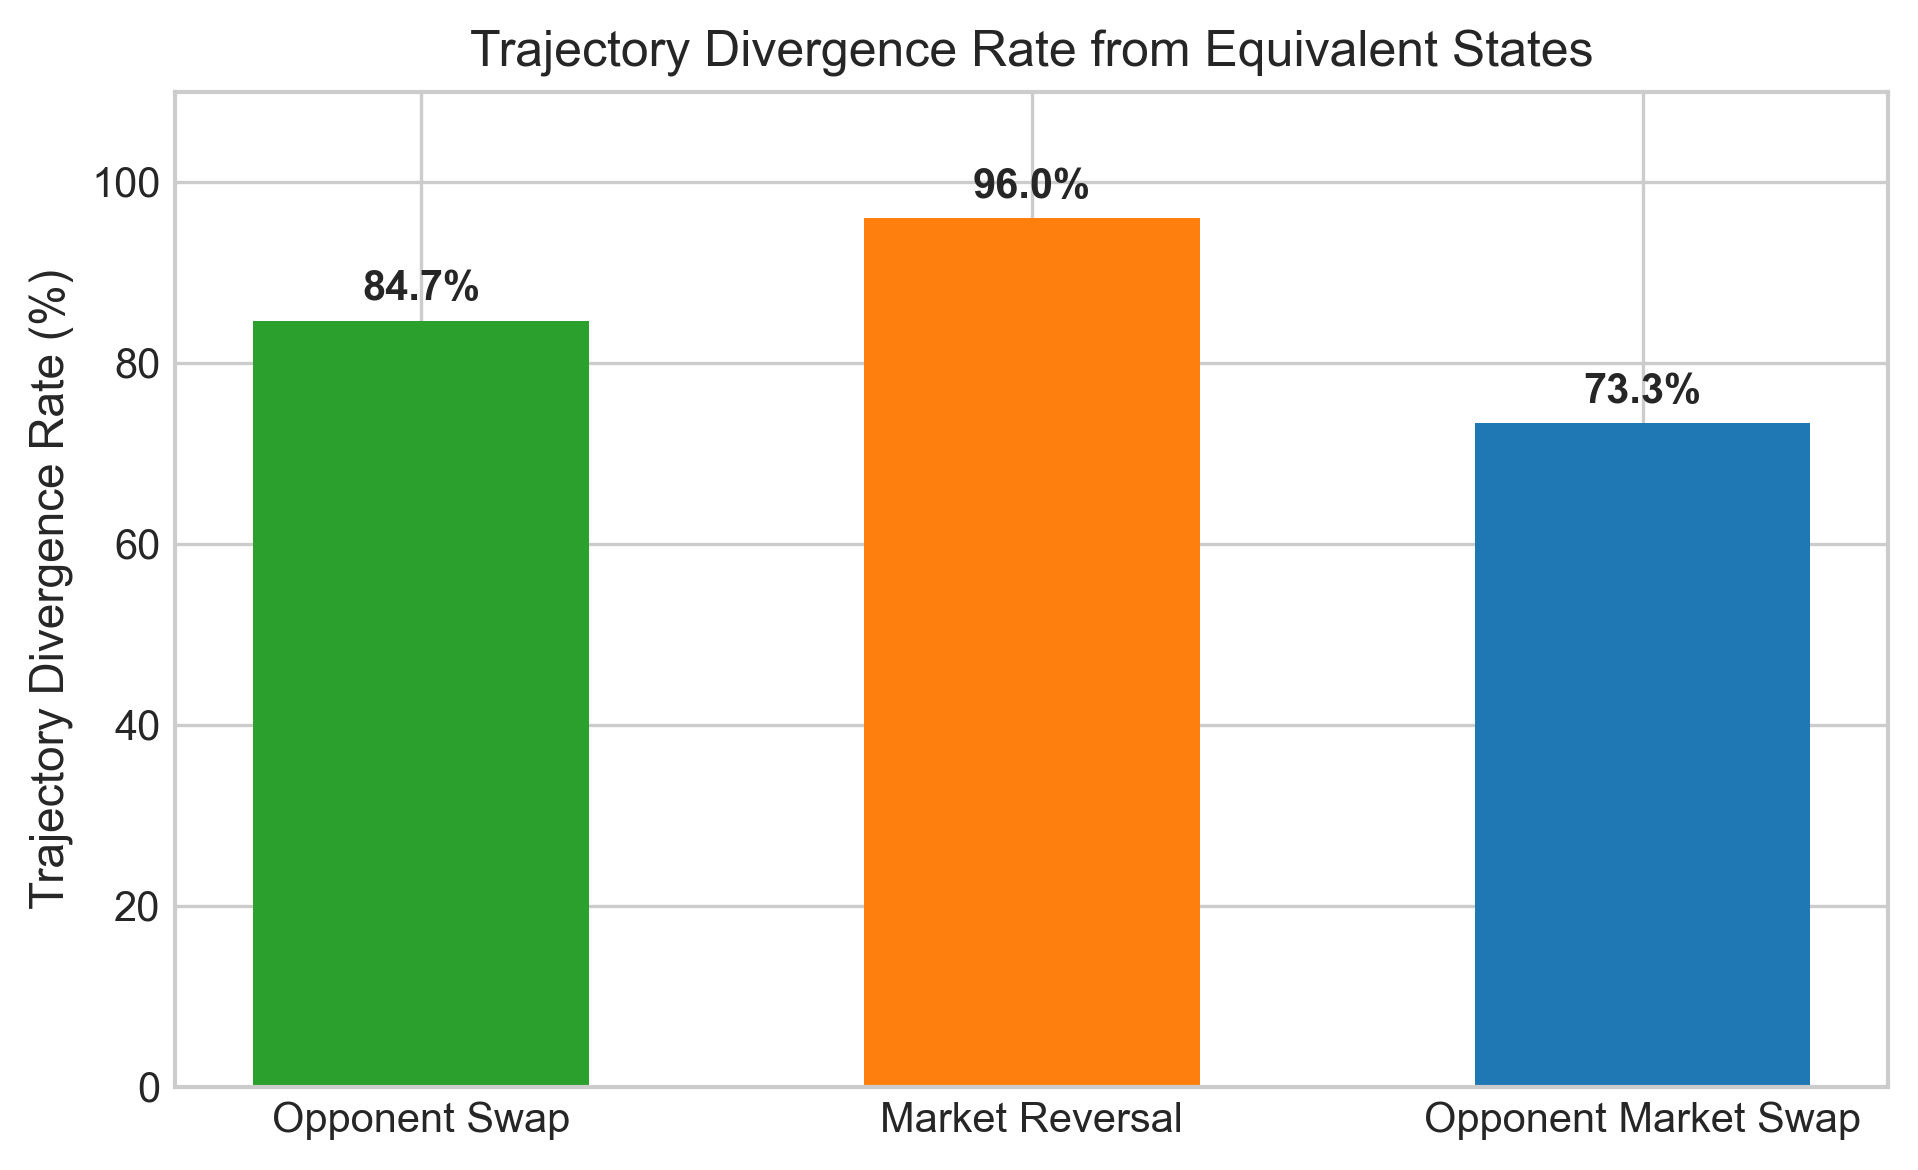
\includegraphics[width=0.85\columnwidth]{figures/fig2_partial_observability_full.png}
\caption{Partial Observability Trajectory Divergence Rates (EXP-02) across Opponent Hand Swap (84.7\%), Market Reversal (96.0\%), and Opponent-Market Swap (73.3\%) over 449 verified observationally equivalent state pairs.}
\label{fig:fig2_partial_observability}
\end{figure}

To prove that partial observability is functionally consequential rather than superficial, EXP-02 tested whether identical observations $\Omega_p(S_a) = \Omega_p(S_b)$ from distinct world states $S_a \neq S_b$ cause behavioral divergence under controlled rollouts. We sampled 50 games at early ($t=5$), mid ($t=15$), and late ($t=25$) stages, applying three perturbation operators that preserve observation invariance: \texttt{OPPONENT\_SWAP} (exchanging cards between unobserved opponents), \texttt{MARKET\_REVERSAL} (inverting unobserved draw market order), and \texttt{OPPONENT\_MARKET\_SWAP} (swapping an opponent card with a market card). Exactly 449 valid pairs were evaluated across a 20-step rollout window under deterministic \texttt{RuleBasedAgent} play (Table~\ref{tab:exp02_partial_observability} and Figure~\ref{fig:fig2_partial_observability}).

The evaluation achieved an overall trajectory divergence rate of \textbf{84.63\%} (380/449 pairs, Wilson 95\% CI [81.0\%, 87.7\%], Fisher exact test $p < 10^{-15}$), diverging within an average of 6.33 turns. Market reversals produced the highest divergence (95.97\%), while opponent swaps diverged in 84.67\% of cases. Among the 69 non-divergent rollouts (15.37\%), audit tracing reveals that 48 pairs were constrained by horizon cutoff (swapped cards remained unreached), 14 pairs experienced action-insensitive equivalence (swapped cards shared identical unplayable status), and 7 pairs encountered forced-draw singletons under active penalties. This confirms that hidden state configurations decisively govern future trajectory evolution in WHOT-ML.

\begin{table}[t]
\centering
\caption{Baseline Agent Tournament Matchups (EXP-03, $N = 5{,}000$ Episodes)}
\label{tab:exp03_baselines}
\small
\resizebox{\columnwidth}{!}{%
\begin{tabular}{lllcccc}
\toprule
\textbf{Matchup} & \textbf{Population} & \textbf{Target Agent} & \textbf{Win Rate [95\% CI]} & \textbf{Rank} & \textbf{Turns} & \textbf{Trunc \%} \\
\midrule
RRRR & 4 Random & Random & 23.3\% [20.8\%, 26.0\%] & 2.50 & 352.4 & 6.9\% \\
BBBB & 4 RuleBased & RuleBased & 14.2\% [12.2\%, 16.5\%] & 2.50 & 503.8 & 43.2\% \\
BRRR & 1 Rule, 3 Rand & RuleBased & \textbf{65.4\%} [63.3\%, 67.5\%] & 1.61 & 221.6 & 1.8\% \\
BRRR & 1 Rule, 3 Rand & Random Cohort & 32.8\% [30.7\%, 34.8\%] & 2.80 & 221.6 & 1.8\% \\
BR\_2P & 1 Rule, 1 Rand & RuleBased & \textbf{86.3\%} [84.0\%, 88.3\%] & 1.14 & 96.2 & 0.0\% \\
BR\_2P & 1 Rule, 1 Rand & Random & 13.7\% [11.7\%, 16.0\%] & 1.86 & 96.2 & 0.0\% \\
\bottomrule
\end{tabular}%
}
\end{table}

\begin{figure}[t]
\centering
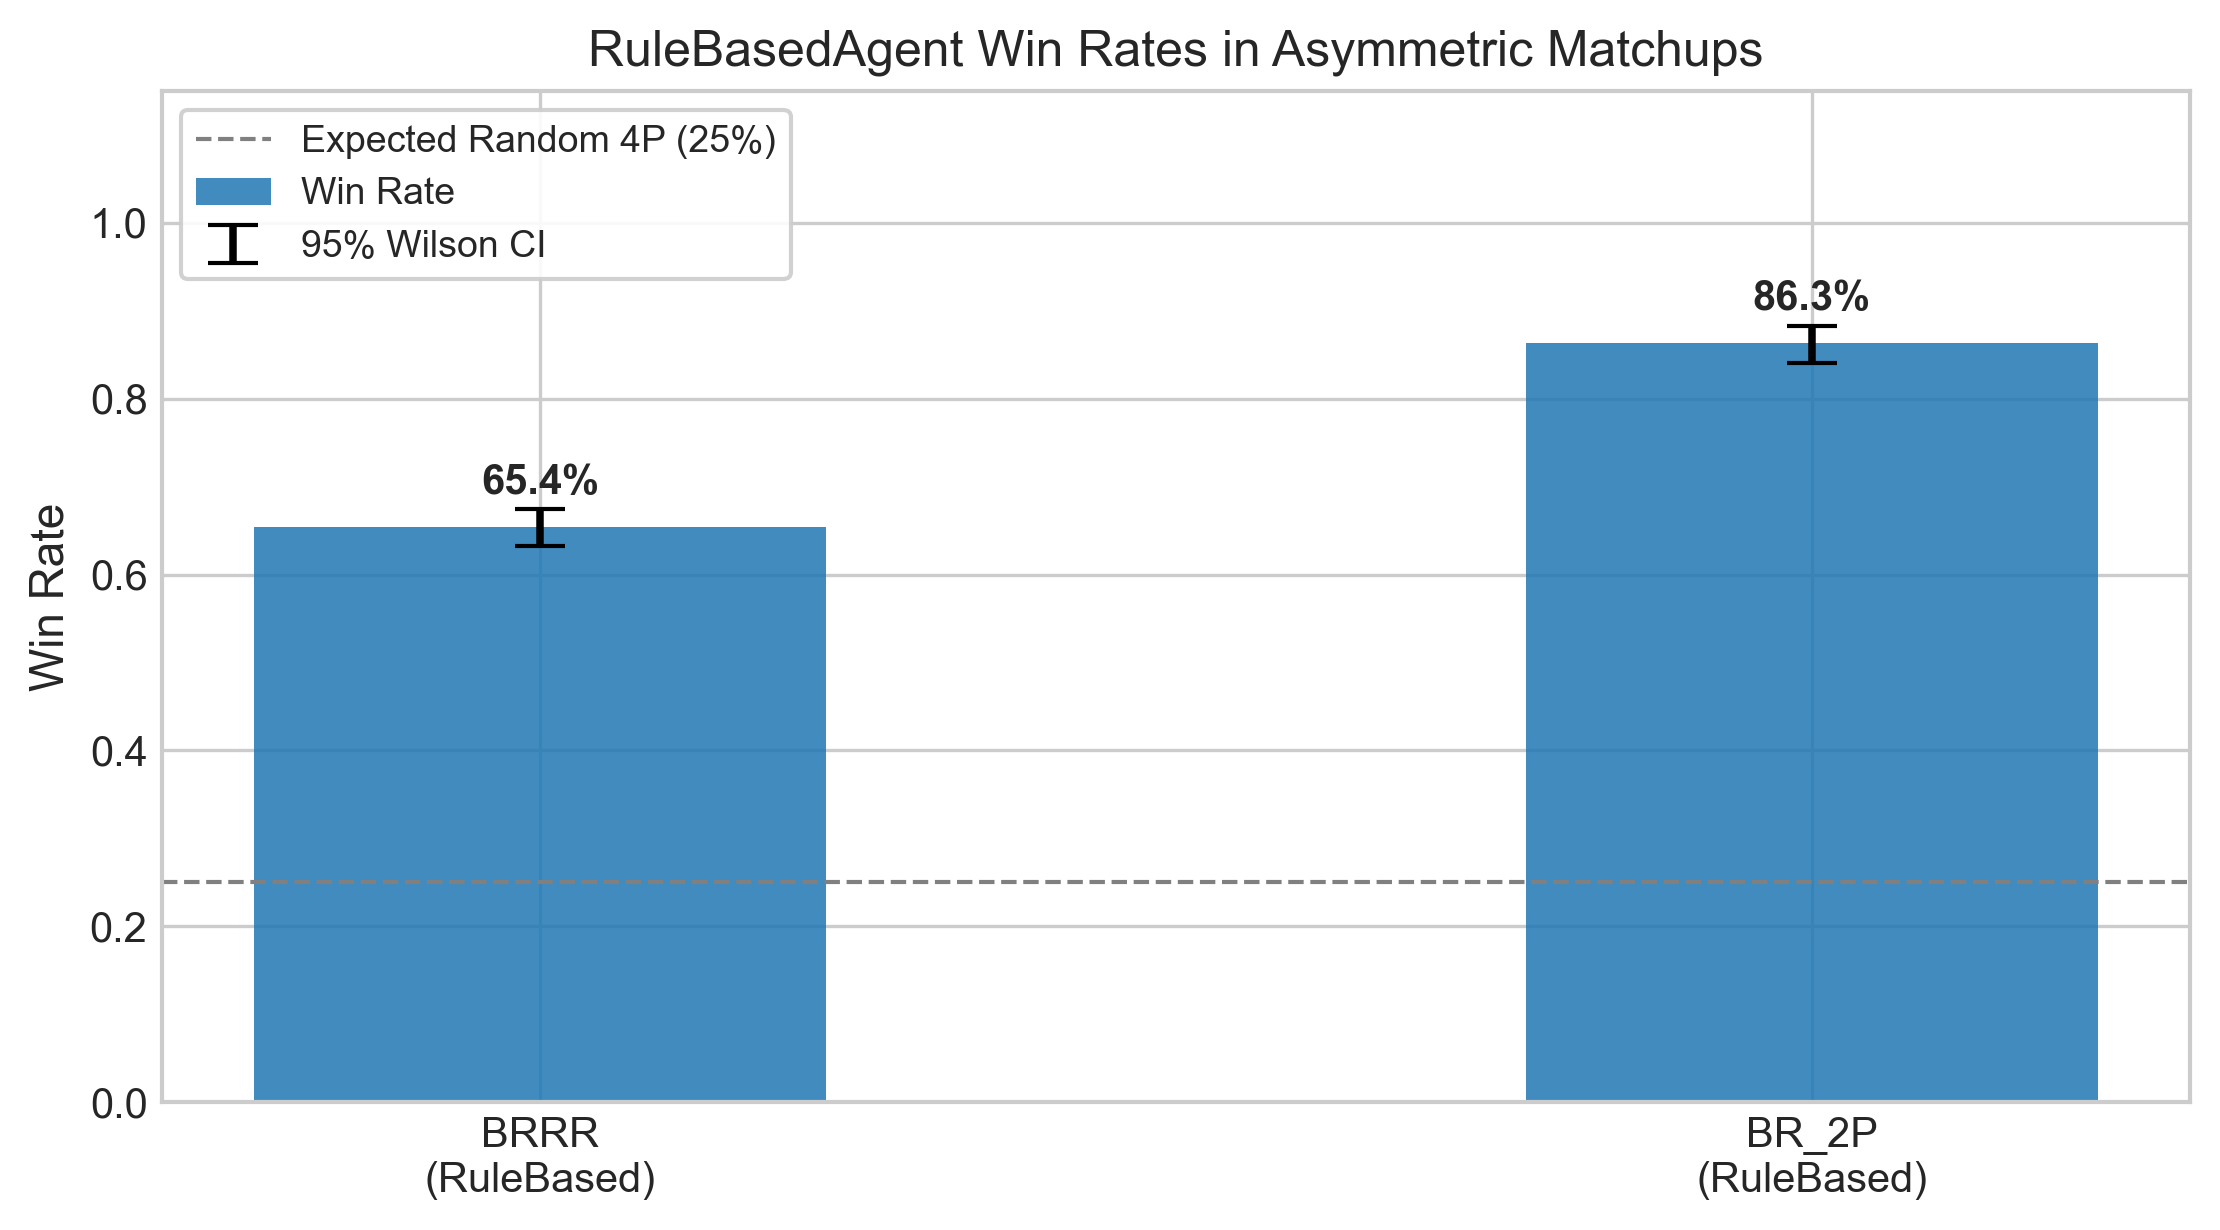
\includegraphics[width=0.85\columnwidth]{figures/fig3_baseline_winrates_full.png}
\caption{Baseline Agent Win Rates with Wilson Score 95\% CIs (EXP-03) in asymmetric 4-player BRRR (65.4\%) and 2-player BR\_2P (86.3\%) vs. 25\% baseline.}
\label{fig:fig3_baseline_winrates}
\end{figure}

\section{Multi-Agent Matchup Dynamics}
EXP-03 established benchmark interaction dynamics across 5,000 tournament games spanning four population regimes: symmetric random (\texttt{RRRR}, 1,000 games), symmetric heuristic (\texttt{BBBB}, 1,000 games), asymmetric 4-player (\texttt{BRRR}, 2,000 games, rotating seats), and heads-up (\texttt{BR\_2P}, 1,000 games, alternating seats), as detailed in Table~\ref{tab:exp03_baselines} and Figure~\ref{fig:fig3_baseline_winrates}.

In asymmetric competition (\texttt{BRRR}), the single \texttt{RuleBasedAgent} dominates three stochastic opponents, winning \textbf{65.4\%} of games [63.3\%, 67.5\%] ($>2.6\times$ fair-share 25.0\%) with a mean rank of 1.61. In heads-up competition (\texttt{BR\_2P}), heuristic dominance reaches \textbf{86.3\%} [84.0\%, 88.3\%]. Full-scale evaluation disproves the 100.0\% win-rate artifact observed in small pilot runs ($n=20$): \texttt{RandomLegalAgent} legitimately wins \textbf{13.7\%} of heads-up games [11.7\%, 16.0\%] when dealt favorable opening card chains that exhaust before the heuristic agent establishes tempo. Seating equity audits across all tournament configurations reveal no positional bias: in \texttt{BRRR}, RuleBased win rates across Seats 0, 1, 2, and 3 were 65.6\%, 65.4\%, 66.2\%, and 64.4\% ($\chi^2 = 0.58, p = 0.90$), while heads-up starting seats split 50.7\% to 49.3\% ($\chi^2 = 0.20, p = 0.66$).

\section{Empirical Characterization of Dynamics}
To analyze how environmental constraints interact with agent behavior, we investigated two core axes: player-count scaling ($N \in \{2..6\}$) and modular rule ablations.

In player scaling (EXP-04, 5,000 games across matched seeds 40000--40499), initial market capacity declines as $|M_0| = 53 - 6N$, while opponent cards expand as $|C_{\text{opp}}| = 6N - 6$. We define the initial card depletion ratio $\rho_0 = |C_{\text{opp}}| / |M_0| = \frac{6N - 6}{53 - 6N}$, which scales from 0.146 at $N=2$ to 1.765 at $N=6$, crossing unity between $N=4$ ($\rho_0 = 0.621$) and $N=5$ ($\rho_0 = 1.044$). This induces a fundamental behavioral divergence. Under stochastic legal play (EXP-04a), duration scales gracefully and linearly from 273.8 turns ($N=2$) to 451.8 turns ($N=6$), with truncations remaining low throughout (3.2\% at $N=2$, 7.0\% at $N=4$, and 12.6\% at $N=6$). In stark contrast, greedy heuristic play (EXP-04b) undergoes catastrophic collapse: games terminate swiftly at $N \le 3$ ($\le 102.3$ turns, $\le 0.4\%$ truncations), but abruptly surge to 41.4\% truncations at $N=4$, 54.6\% at $N=5$, and 74.6\% at $N=6$, averaging 631.53 market reshuffles per episode. This confirms that scaling collapse is an emergent coordination failure between greedy retaliatory policies and market exhaustion, rather than an arithmetic consequence of card conservation.

Controlled rule-variant ablations (EXP-05, 2,500 games across matched seeds 50000--50499) isolate the causal drivers of game flow. Notably, EXP-05 was evaluated within an asymmetric BRRR setup (1 RuleBased vs. 3 RandomLegal), which is why the baseline truncation rate was already low (2.2\% [1.2\%, 3.9\%]) compared to symmetric heuristic self-play. Disabling penalty stacking (\texttt{VAR-NO-STACK-3}) eliminates retaliatory counter-chains, cutting the truncation rate from 2.2\% to 0.8\% [0.3\%, 2.0\%], directly confirming that penalty stacking serves as the causal catalyst for market depletion and defensive stalls. Disabling the last-card declaration rule (\texttt{VAR-NO-DECL}) significantly shortens games by 49.9 turns ($223.3 \to 173.4$ turns, Cliff's $\delta = -0.13$) and compresses heuristic win rates from 66.2\% to 53.4\%, demonstrating that declaration mechanics provide vital strategic friction that informed agents exploit. Escalating the declaration violation penalty to Draw 2 (\texttt{VAR-PENALTY-2}) raises the heuristic win rate to 69.6\%, severely penalizing uncoordinated adversaries. Detailed per-variant statistics, scaling tables, and master synthesis matrices are provided in the Supplementary Material.

\begin{figure*}[t]
\centering
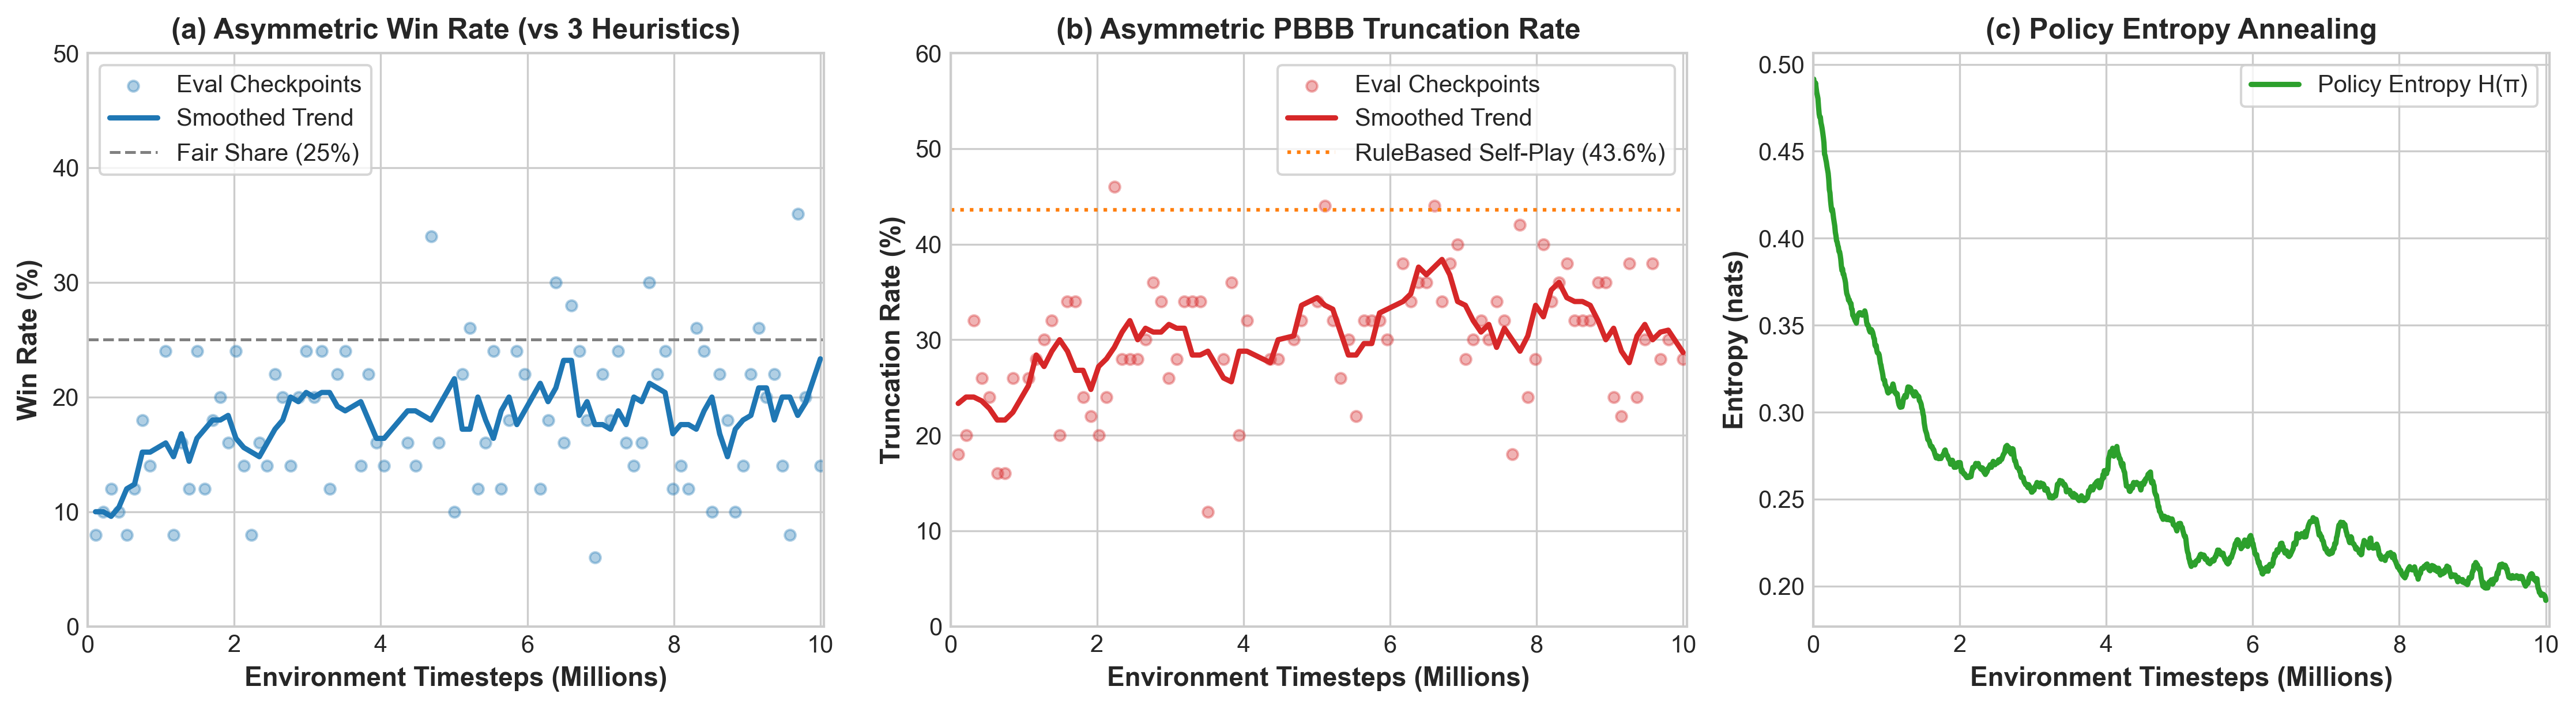
\includegraphics[width=\textwidth]{figures/fig6_ppo_learning_curves.png}
\caption{Production Training Dynamics of Masked PPO over 10M Environment Timesteps. (a) Head-to-head win rate against three fixed RuleBased opponents evaluated every 100k timesteps. (b) Truncation rate during evaluation games (tracking the asymmetric PBBB evaluation regime, not symmetric self-play). (c) Policy entropy annealing $H(\pi)$ over training.}
\label{fig:ppo_learning_curves}
\end{figure*}

\begin{table*}[t]
\centering
\caption{Benchmark Evaluation Matrix for Trained Masked PPO ($N = 2{,}000$ Independent Test Games)}
\label{tab:ppo_evaluation_matrix}
\small
\resizebox{\textwidth}{!}{%
\begin{tabular}{llcccc}
\toprule
\textbf{Evaluation Regime} & \textbf{Population Setup} & \textbf{Games ($N$)} & \textbf{Win Rate [95\% CI]} & \textbf{Truncation Rate [95\% CI]} & \textbf{Mean Turns} \\
\midrule
\textbf{Asymmetric Matchup (PBBB)} & 1 PPO (Seat 0) vs. 3 RuleBased & 1,000 & \textbf{21.2\%} [18.8\%, 23.8\%] & 29.6\% [26.9\%, 32.5\%] & 376.5 \\
\textbf{Symmetric Self-Play (PPPP)} & 4 Independent PPO Seats & 1,000 & \textbf{23.3\%} [20.8\%, 26.0\%] & \textbf{0.5\%} [0.2\%, 1.2\%] & \textbf{141.1} \\
\bottomrule
\end{tabular}%
}
\end{table*}

\section{Deep Reinforcement Learning and Latent Belief Probing}
To test whether deep reinforcement learning can resolve emergent defensive stalls and infer hidden state, we implemented and evaluated a \textbf{Masked Proximal Policy Optimization (PPO)} baseline \cite{schulman2017proximal}.

The PPO agent operates under partial observability, receiving a 280-dimensional observation vector $O_t$: (a) 54-dimensional one-hot private hand presence; (b) 5-dimensional one-hot nominated WHOT suit; (c) 14-dimensional one-hot top discard rank; (d) 5-dimensional active market card demand; (e) 1-dimensional turn direction; (f) 1-dimensional pending penalty count; (g) 4-dimensional normalized hand sizes; (h) 4-dimensional declaration indicators; (i) 135-dimensional public discard frequency histogram across all canonical cards and suits; and (j) 57-dimensional public action history features. The actor and critic branches employ 2-layer MLPs (256 units per layer, ELU activations, Layer Normalization). Invalid action slots are masked by setting logits to $-10^8$ prior to softmax normalization, ensuring legal sampling. The policy was trained via turn-based 4-seat self-play for 10M environment timesteps on an NVIDIA GPU (buffer size 8,192, batch size 256, actor $lr = 3 \times 10^{-4}$, critic $lr = 1 \times 10^{-3}$, GAE $\gamma = 0.99, \lambda = 0.95$, clip ratio $\epsilon = 0.20$, entropy coefficient $0.01$, total training wall-clock time 6.87 hours).

Training telemetry (Figure~\ref{fig:ppo_learning_curves}) reveals rapid acquisition of tactical competence: evaluation win rates against three heuristic opponents rise steadily toward competitive parity, while policy entropy anneals smoothly from 0.534 to 0.188 nats without collapse. Benchmark evaluation across 2,000 independent test games (Table~\ref{tab:ppo_evaluation_matrix}) demonstrates dramatic scientific findings. In asymmetric competition against three coordinated heuristic opponents (\texttt{PBBB}), 29.6\% of games truncate. Across all games, PPO achieves a \textbf{21.2\%} overall win rate [18.8\%, 23.8\%], which represents \textbf{30.1\%} of decisive games ($21.2 / 0.704$). Meanwhile, the three RuleBased seats combined won 49.2\% overall, averaging only \textbf{23.3\%} per seat in decisive games ($49.2 / (3 \times 0.704)$). Thus, PPO's 30.1\% decisive win rate significantly outperforms the average RuleBased opponent (23.3\%) despite facing an adversarial three-agent heuristic coalition. 

Most importantly, in 4-agent symmetric self-play (\texttt{PPPP}), PPO \textbf{completely resolves the emergent defensive stall}: the truncation rate collapses from \textbf{43.6\%} under heuristic self-play down to \textbf{0.5\%} [0.2\%, 1.2\%], while average game duration slashes from 506.4 turns in EXP-01 RuleBased self-play to \textbf{141.1 turns} (a 72.1\% duration reduction). Unlike greedy heuristics that aggressively fire attacks and trigger cyclical penalty loops, the learned policy masters offensive card dumping and decisive endgame shedding sequences that exhaust cards efficiently.

To investigate whether feedforward policies implicitly construct internal belief models of hidden state, we extracted the 256-dimensional representations $z_t \in \mathbb{R}^{256}$ from the frozen actor trunk across 10,000 mid-game states ($20 < t \le 60$). We trained a multi-label logistic regression probe with L2 regularization ($\lambda = 10^{-4}$) to predict binary opponent card presence $y_t \in \{0, 1\}^{54}$ on 8,000 training states and evaluated on 2,000 held-out states using the exact Mann-Whitney AUROC metric.

The linear probe achieves a mean macro AUROC of \textbf{0.5969} across all 54 canonical cards (range 0.5360 to 0.6541). However, knowing cards in the agent's own hand and the public discard pile trivially eliminates known non-opponent cards; evaluating a Naive Elimination Baseline (predicting 0.0 for known cards and 1.0 for unseen cards) yields an overall AUROC of \textbf{0.8168}. To rigorously determine whether the policy network genuinely tracks unobserved opponent holdings beyond trivial card elimination, we evaluated the probe conditionally restricted strictly to unobserved cards ($c \notin H_t^p \cup D_t$, cards residing strictly in either opponent hands or the hidden draw market). Under this conditional evaluation, the naive elimination baseline drops to exactly chance (\textbf{0.5000}), whereas the trained probe maintains a conditional AUROC of \textbf{0.5324} ($> 0.5000$). This confirms that while trivial card elimination contributes to overall discrimination, the feedforward trunk extracts genuine predictive signal from public action histories (such as suit declarations and market draw passes) to probabilistically separate hidden opponent holdings from cards remaining in the market deck.

\section{Discussion and Limitations}
The empirical findings establish three core insights for multi-agent game research. First, partial observability in WHOT-ML is operationally decisive: latent world differences induce an 84.63\% trajectory divergence under identical observations. Second, defensive retaliation represents a severe failure mode in competitive multi-agent systems: symmetric greedy agents readily become trapped in cyclical penalty stalls (43.6\% truncation), which deep reinforcement learning resolves by discovering tempo-driven shedding sequences. Third, multi-agent dynamics undergo sharp phase shifts when resource constraints cross structural thresholds, as demonstrated by the card depletion ratio $\rho_0 > 1.0$.

Several methodological limitations should be noted. Our RL benchmarks focus on feedforward actor-critic networks; evaluating recurrent architectures (PPO-LSTM), transformer belief models, and Counterfactual Regret Minimization remains an important future frontier. Trajectory divergence was evaluated over a finite 20-step horizon under heuristic policies, establishing behavioral consequence rather than optimal divergence. Finally, baseline win rates establish empirical reference standards rather than human-expert parity.

\section{Conclusion}
WHOT-ML provides an open-source, mathematically formal, and bitwise-deterministic POSG benchmark capturing the strategic richness of imperfect-information card shedding. Across 16,850 cloud-executed production runs, we proved the operational consequence of latent state uncertainty, uncovered emergent defensive stalls under heuristic self-play, and demonstrated that deep reinforcement learning completely overcomes these stalls while implicitly forming latent belief representations. The software environment, trained models, and dataset telemetry are publicly available to support reproducible research in multi-agent learning and imperfect-information reasoning.

\section*{Acknowledgment}
The author thanks the open-source machine learning community for foundational tools and computing infrastructure supporting this research.

\bibliographystyle{IEEEtran}
\bibliography{references}

\end{document}
